
\documentclass[preprint,12pt,notitlepage]{elsarticle}

\usepackage[spanish]{babel}
\usepackage{amssymb}
\usepackage{graphicx}
\usepackage{lineno}
\usepackage[utf8]{inputenc}
\usepackage{url}
\usepackage{natbib}

\begin{document}
	
	\begin{frontmatter}

		\title{\huge  PROYECTO DE  ANALISIS Y  MEJORAMIENTO DE  SOFTWARE }
		\author{Katerin Merino Quispe  (2018060918)}
		\author{Percy Taquila Carazas  (2018061088)}
		\author{Abraham Lipa Calabilla (2019064039)}
		\author{Edwart                ()}
		\author{Liz                ()}
		\address{Tacna, Perú}
		
%%INICIO abstract
\begin{abstract}
This document is intended to present patient care in a concise and clear way, diagnosing their possible disease with terms of software that would be carried out in the system. In this documentation, the requirements that will serve as a guide to develop the software in its different stages will be reflected, helping us to validate and inspect its construction, applying the Software quality.

Therefore, we will work with Sonarqube for the analysis of static code to analyze the code and find code errors, and security vulnerabilities. SonarSource's C Sharp analysis has extensive coverage of well-established quality standards.  
\end{abstract}
%%FIN abstract

\end{frontmatter}

\section*{Resumen}

Este documento tiene como objetivo presentar la atención al paciente de forma concisa y clara, diagnosticando su posible enfermedad con términos de software que se llevarían a cabo en el sistema. En esta documentación se reflejarán los requisitos que nos servirán de guía para desarrollar el software en sus diferentes etapas, ayudándonos a validar e inspeccionar su construcción, aplicando la calidad del Software.

Por lo tanto, trabajaremos con Sonarqube para el análisis de código estático para analizar el código y encontrar errores de código y vulnerabilidades de seguridad. El análisis C Sharp de SonarSource tiene una amplia cobertura de estándares de calidad bien establecidos.

%%INICIO Introducción
\section{Antecedentes o Introducción}

El Sistema de Diagnostico Médico está desarrollado para que la atención a los pacientes sea mas rápida, ya que en esta pandemia hace que la atencion sea insufiente, por falta de tiempo y con este sistema se busca una atencion mas rápido y de forma ordenada, a los pacientes que vienen para hacer sus consultas. Con este sistema se diagnostica al paciente con los síntomas que nos diga en el momento de la consulta y dar como resultado la posible enfermedad que padece.
%%FIN Introducción

%%INICIO Titulo
\section{Titulo}
"Sistema de Diagnostico Médico"

Propuesta de un sistema de atención al paciente diagnosticando su posible enfermedad.
%%FIN Titulo
%%INICIO Autores
\section{Autores}
\begin{itemize}
    \item Katerin Merino Quispe
    \item Abraham Lipa Calabilla
    \item Percy Taquila Carazas
    
\end{itemize}
%%FIN Autores
%%INICIO Planteamiento del problema
\section{Planteamiento del problema}
%%----------------------------------------------------------------------------------------------------------------------------------------------------------
	\subsection{\textbf{Problema}}
Falta e insuficiencia de herramientas para el apoyo en el diagnóstico medico de enfermedades, además por la pandemia que está pasando el mundo entero la demanda de pacientes no está siendo cubierta. Es por ello que muchos pacientes no son atendidos y por esta razon se necesita un sistema que apoye en el diagnostico, para poder agilizar la atención hacia los pacientes.
%%-----------------------------------------------------------------------------
	\subsection{\textbf{Justificación }}
Crear un sistema de diagnóstico para las enfermedades es necesario debido a que puede ayudar al medico a brindar una respuesta más rápida, la implementación de este sistema va a mejorar la gestión de los servicios y la atención.

%%-----------------------------------------------------------------------------
	\subsection{\textbf{ Alcance }}
El software a desarrollar servira de apoyo para poder diagnosticar algunas enfermedades de acuerdo a los sintomas que el paciente presente.

\section{Objetivos}
	\subsection{\textbf{ General }}
		\begin{itemize}
			\item Desarrollar un sistema de diagnóstico médico para optimizar el tiempo de respuesta del diagnóstico médico.
		\end{itemize}
	\subsection{\textbf{Específicos }}

\begin{itemize}
	\item Que el diagnóstico médico muestre las posibles enfermedades de un paciente.
	\item Detectar que tipo de posible enfermedad tiene el paciente. 
	\item Almacenar el historial del paciente en la base de datos. 
\end{itemize}

\section{Referentes teóricos}

\subsection{Título:} Sistema Experto para el Diagnóstico de Enfermedades Respiratorias en el Hospital Central de la Policía Nacional del Perú Luis N. Sáenz

\subsection{Autor(es):} Harold Anderson Chacaltana La Rosa

\subsection{Año:} 2017

\subsection{Resumen:}

El objetivo principal del presente trabajo es crear un sistema experto para el diagnóstico de enfermedades respiratorias, el cual será utilizado inicialmente en el Área de Neumología del Hospital Central PNP Luis N. Sáenz; permitiendo con ello atender de manera inmediata las inquietudes de los pacientes. El principal problema que afronta la institución es la carencia de personal médico especializado en el rubro de neumología, para atender a más de 500 pacientes al día, tal situación se complica aún más por la carencia de un sistema informático para el apoyo del diagnóstico.

El presente trabajo de investigación se realiza con la finalidad de aminorar los tiempos de respuesta del diagnóstico de las enfermedades respiratorias; debido a la afluencia de pacientes los médicos no se dan abasto en la atención, demorando en analizar los síntomas, por lo tanto, el tiempo de consulta es mayor; como consecuencia la atención es más prolongada de lo esperado, generando la reducción de pacientes a atender.

En el área de neumología debido al clima, la cantidad de incidentes va en aumento,a ello se suma la contaminación ambiental, y el poco personal especializado para la atención. [...]

\subsection{Autor(es):} Marlene Carlos Soto

\subsection{Año:} 2002

\subsection{Título:} Sistema Experto de Diagnostico Médico del Síndrome de Guillian Barre

\subsection{Resumen:}

[...] De esta manera esta monografía de Tesis tratará en el Capitulo 1: Teoría de Sistemas Expertos lo concerniente al fundamento teórico de los Sistemas Expertos: historia, definición, razones para la utilización de un Sistema Experto, los componentes que tiene, las áreas de aplicación de estos Sistemas y los tipos en los que se han clasificado estos sistemas. También se explicará la metodología existente para la confección de Sistemas Expertos.

En el Capitulo II: Técnicas Aplicadas a Sistemas Expertos, se verá como se representa el conocimiento para la implementación de un sistema experto, así como los métodos de resolución de problemas para las formas de representación más conocidas. En este capítulo se explicarán las Redes Neuronales, conceptos, Historia, Clasificación, Aplicaciones y el Algoritmo de Diagnóstico utilizando las Redes Neuronales.

En el Capitulo III: Síndrome de Guillian Barre y su diagnóstico se desarrollará el tema de aplicación de esta tesis, antes de ello se explicará como el médico llega a un diagnóstico y luego se verá la enfermedad, síntomas y su diagnóstico.

En el Capitulo IV: Un Sistema Experto para el diagnóstico del Síndrome Guillian Barre se explicará la aplicación realizada, la base de conocimiento, y el algoritmo utilizado para la solución del problema. [...]

\section{Desarrollo de la propuesta}
La calidad de código suele decirse que es un atributo interno de calidad, dado que no se hace visible al usuario. Pero llega un momento en el cual este atributo de calidad pasa de ser interno a externo, y esto se da cuando el hecho de tener modificar el código para hacer un cambio lleva mucho más tiempo del que debería. Con el fin de verificar la calidad interna de un sistema se suelen hacer análisis de código con SonarQube o herramientas similares. En este documento se muestra parte de de nuestro proyecto , donde básicamente cuenta cómo hacer una prueba de concepto rápidamente usando una imagen Docker de SonarQube, y ejecutando el análisis desde SonarQube Scanner.
SonarQube, como tantas otras herramientas similares, permite realizar análisis estático de código fuente de manera automática, buscando patrones con errores, malas prácticas o incidentes. Además, realiza un cálculo de la deuda técnica. Dentro de las verificaciones que hacen herramientas como SonarQube, se encuentran las siguientes:
\begin{itemize}
	\item Detección de código duplicado..
	\item Falta de pruebas unitarias, falta de comentarios. 
	\item Código spaghetti, complejidad ciclomática, alto acoplamiento.
	\item Tamaño de archivos de código.
	\item Tamaño de métodos.
	\item No adecuación a estándares y convenciones de código.
	\item Vulnerabilidades conocidas de seguridad.
	
	Una muestra en Nuestro proyecto:
		
\begin{center}
	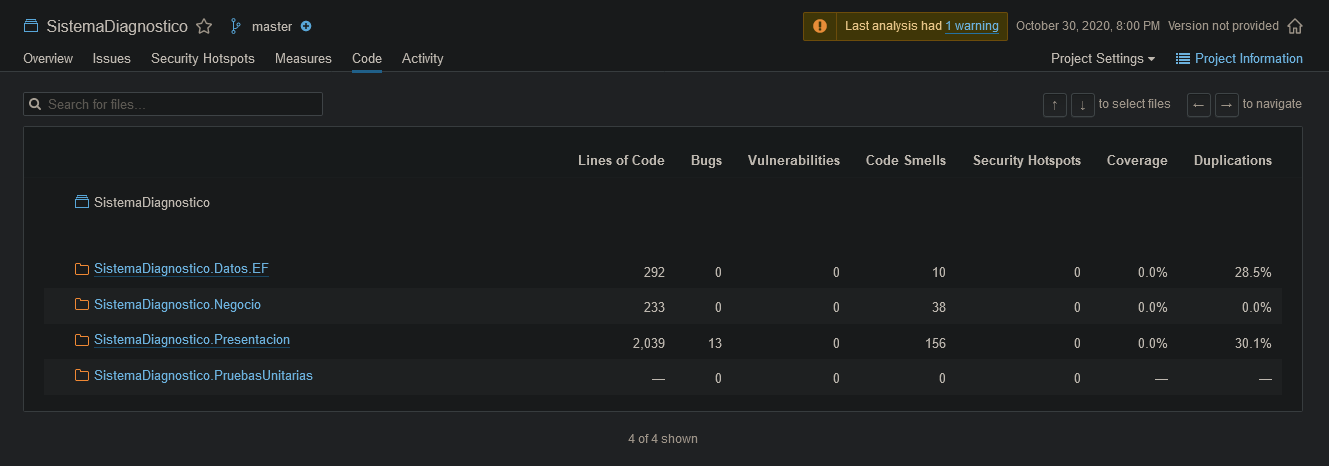
\includegraphics[width=12cm]{./imagen/Screenshot_2020-10-30 Code.png} 
	\end{center}
\end{itemize}

\subsection{\textbf{Tecnología de información  }}
		\begin{itemize}
	\item 	SQL SERVER: Microsoft SQL Server es un sistema de gestión de base de datos relacional, desarrollado por la empresa Microsoft. El lenguaje de desarrollo utilizado es Transact-SQL, una implementación del estándar ANSI del lenguaje SQL, utilizado para manipular y recuperar datos, crear tablas y definir relaciones entre ellas..
	\item 	C-Sharp : lenguaje de programación multiparadigma desarrollado y estandarizado por Microsoft. Es un lenguaje de programación creado para diseñar aplicaciones en la plataforma.NET.
	\item 	Visual Studio: es un entorno de desarrollo en diferentes sistemas operativos y compatibles con múltiples lenguajes de programación al igual que entornos de desarrollo web. 
	\end{itemize}
\subsection{\textbf{ Metodología, técnicas usadas  }}
UML es un lenguaje para hacer modelos y es independiente de los métodos de análisis y diseño. Existen diferencias importantes entre un método y un lenguaje de modelado. Un método es una manera explícita de estructurar el pensamiento y las acciones de cada individuo. Además, el método le dice al usuario qué hacer, cómo hacerlo, cuándo hacerlo y por qué hacerlo; mientras que el lenguaje de modelado carece de estas instrucciones. Los métodos contienen modelos y esos modelos son utilizados para describir algo y comunicar los resultados del uso del método.
          \begin{center}
	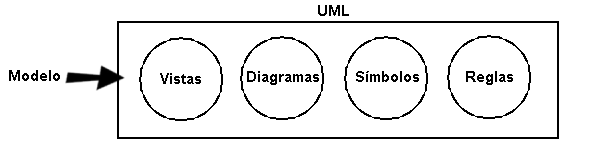
\includegraphics[width=12cm]{./imagen/5} 
	\end{center}
		
\section{Cronograma }
	
	\subsection{Iteraciones}
	\begin{center}
		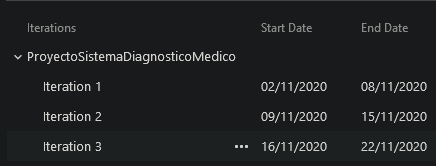
\includegraphics[width=12cm]{./imagen/Screenshot_3.png} 
	\end{center}
	
	\subsection{Tablero de iteraciones y duración}
	\begin{center}
		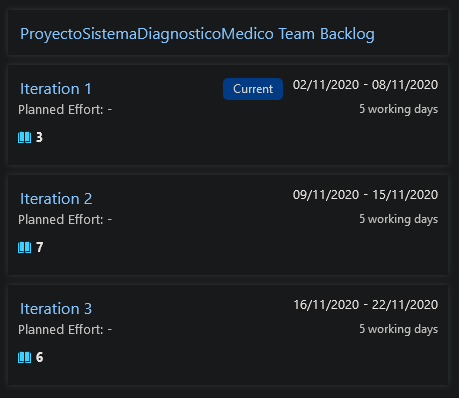
\includegraphics[width=12cm]{./imagen/Screenshot_4.png} 
	\end{center}
	\subsubsection{Iteración 1}
	\begin{center}
	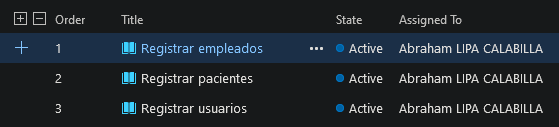
\includegraphics[width=12cm]{./imagen/Screenshot_7.png} 
	\end{center}
	\subsubsection{Iteración 2}
	\begin{center}
	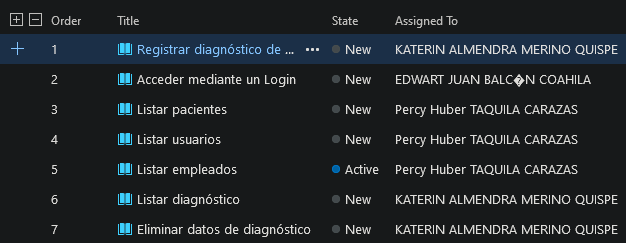
\includegraphics[width=12cm]{./imagen/Screenshot_6.png} 
	\end{center}
	\subsubsection{Iteración 3}
	\begin{center}
	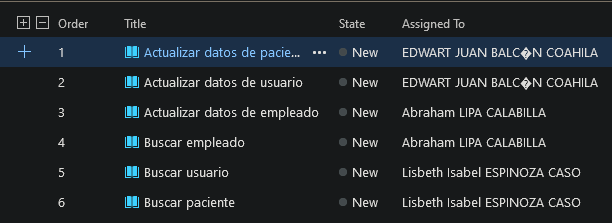
\includegraphics[width=12cm]{./imagen/Screenshot_5.png}
	\end{center}

	\subsubsection{Backlog}
	\begin{center}
	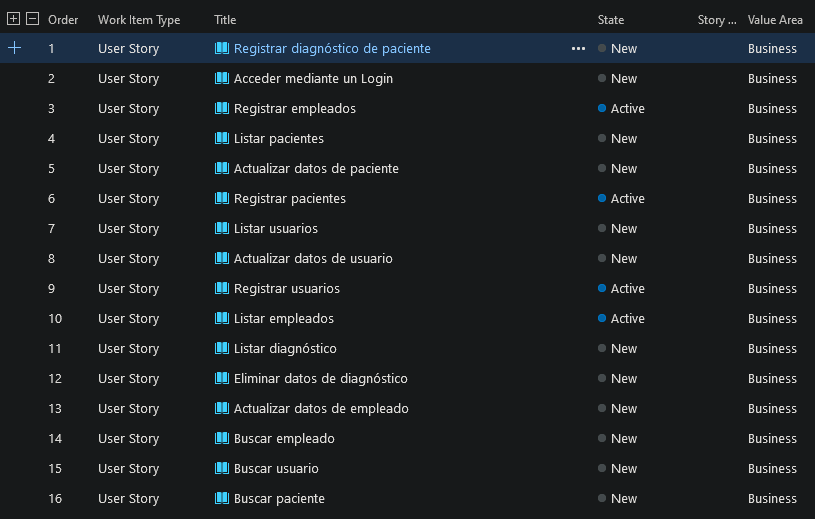
\includegraphics[width=12cm]{./imagen/Screenshot_8.png}
	\end{center}

	\subsection{Tablero de historias}


	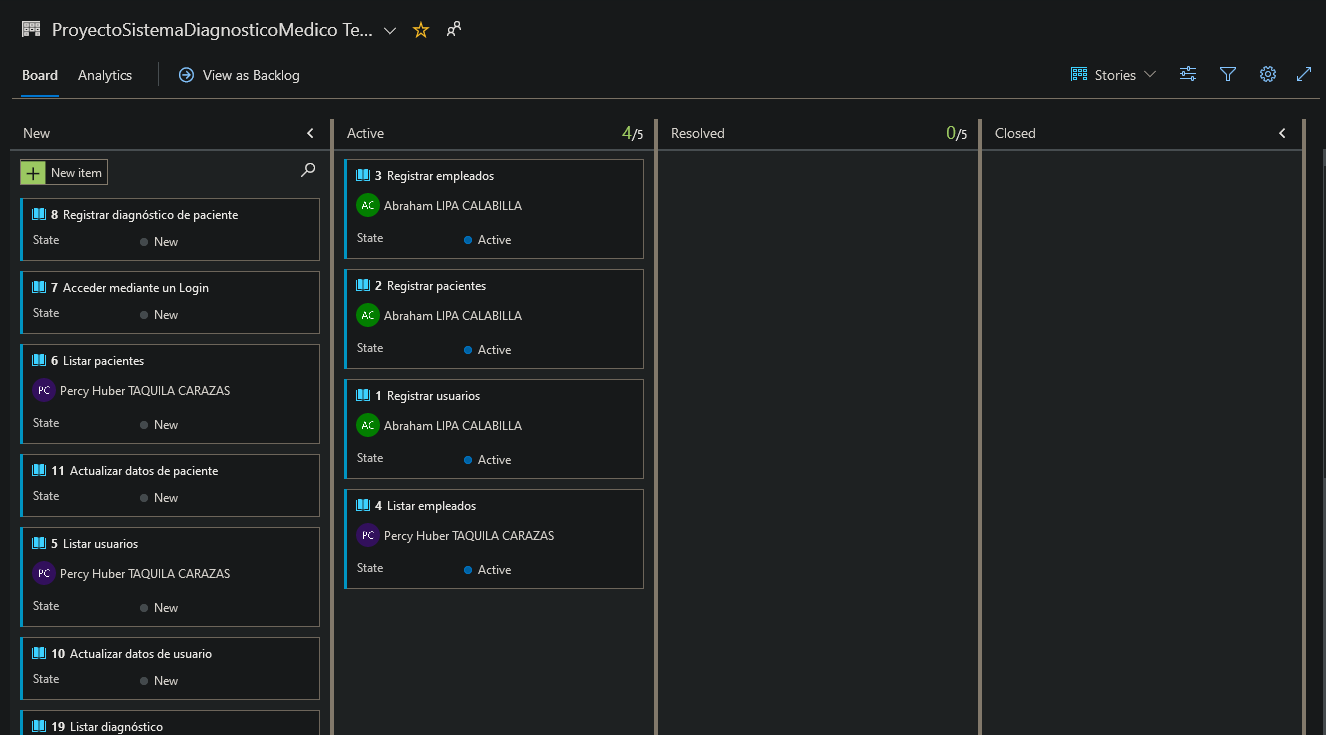
\includegraphics[width=12cm]{./imagen/Screenshot_2020-10-31 ProyectoSistemaDiagnosticoMedico Team Stories Board - Boards.png}




\end{document}

